\documentclass{standalone}
\usepackage{tikz}
\usepackage{ctex,siunitx}
\usepackage{tkz-euclide}
\usepackage{amsmath}
\usetikzlibrary{patterns, calc}
\usetikzlibrary {decorations.pathmorphing, decorations.pathreplacing, decorations.shapes,}
\begin{document}
\small
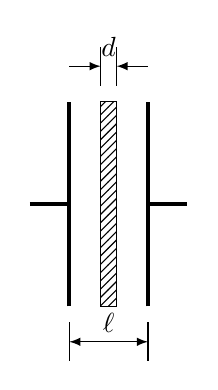
\begin{tikzpicture}[>=latex,scale=1.0]
	\draw[ultra thick] (-0.5,0)--(0,0);
	\draw[ultra thick] (1,0)--(1.5,0);
	\draw [ultra thick] (0,-1.3)--(0,1.3);
	\draw[ultra thick]  (1,-1.3)--(1,1.3);
	\fill [pattern=north east lines, draw ](.4,-1.3) rectangle (.6,1.3);
	\draw (0,-1.5)--(0,-2.0);\draw (1,-1.5)--(1,-2.0);
	\draw [<->](0,-1.75)--(1,-1.75)node[midway,above]{$\ell$};
	\draw (.4,1.5)--(.4,2.0);\draw (.6,1.5)--(.6,2.0);
	\draw [->](0,1.75)--(.4,1.75);
	\draw [->](1,1.75)--(.6,1.75);
	\node at (.5,2.0){$d$};
\end{tikzpicture}
\end{document}